\documentclass[a4paper,10pt]{jsarticle}

% 数式
\usepackage{amsmath,amsfonts}
\usepackage{bm}
% 画像
\usepackage[dvipdfmx]{graphicx}
\usepackage{here}

\usepackage{listingsutf8,jlisting} %日本語のコメントアウトをする場合jlistingが必要
%ここからソースコードの表示に関する設定
\lstset{
  basicstyle={\ttfamily},
  identifierstyle={\small},
  commentstyle={\smallitshape},
  keywordstyle={\small\bfseries},
  ndkeywordstyle={\small},
  stringstyle={\small\ttfamily},
  frame={tb},
  breaklines=true,
  columns=[l]{fullflexible},
  numbers=left,
  xrightmargin=0zw,
  xleftmargin=3zw,
  numberstyle={\scriptsize},
  stepnumber=1,
  numbersep=1zw,
  lineskip=-0.5ex
}

\begin{document}

\title{コンパイラ演習課題}
\author{坪井正太郎(101830245)}
\date{\today}
\maketitle
\section{}
\subsection{1行目終了時点}
\begin{table}[H]
  \centering
  \begin{tabular}{|c|c|c|}
    \hline
    name & kind & val/addr \\ \hline
    x    & var  & 0        \\ \hline
    y    & var  & 1        \\ \hline
    z    & var  & 2        \\ \hline
  \end{tabular}
\end{table}

\subsection{3行目終了時点}
\begin{table}[H]
  \centering
  \begin{tabular}{|c|c|c|}
    \hline
    name & kind  & val/addr  \\ \hline
    x    & var   & 0         \\ \hline
    y    & var   & 1         \\ \hline
    z    & var   & 2         \\ \hline
    exp  & func  & $a_{exp}$ \\ \hline
    x    & param & 0         \\ \hline
    y    & param & 1         \\ \hline
    rv   & var   & 2         \\ \hline
  \end{tabular}
\end{table}

\subsection{8行目終了時点}
\begin{table}[H]
  \centering
  \begin{tabular}{|c|c|c|}
    \hline
    name & kind & val/addr  \\ \hline
    x    & var  & 0         \\ \hline
    y    & var  & 1         \\ \hline
    z    & var  & 2         \\ \hline
    exp  & func & $a_{exp}$ \\ \hline
  \end{tabular}
\end{table}

\section{}
\begin{figure}[H]
  \centering
  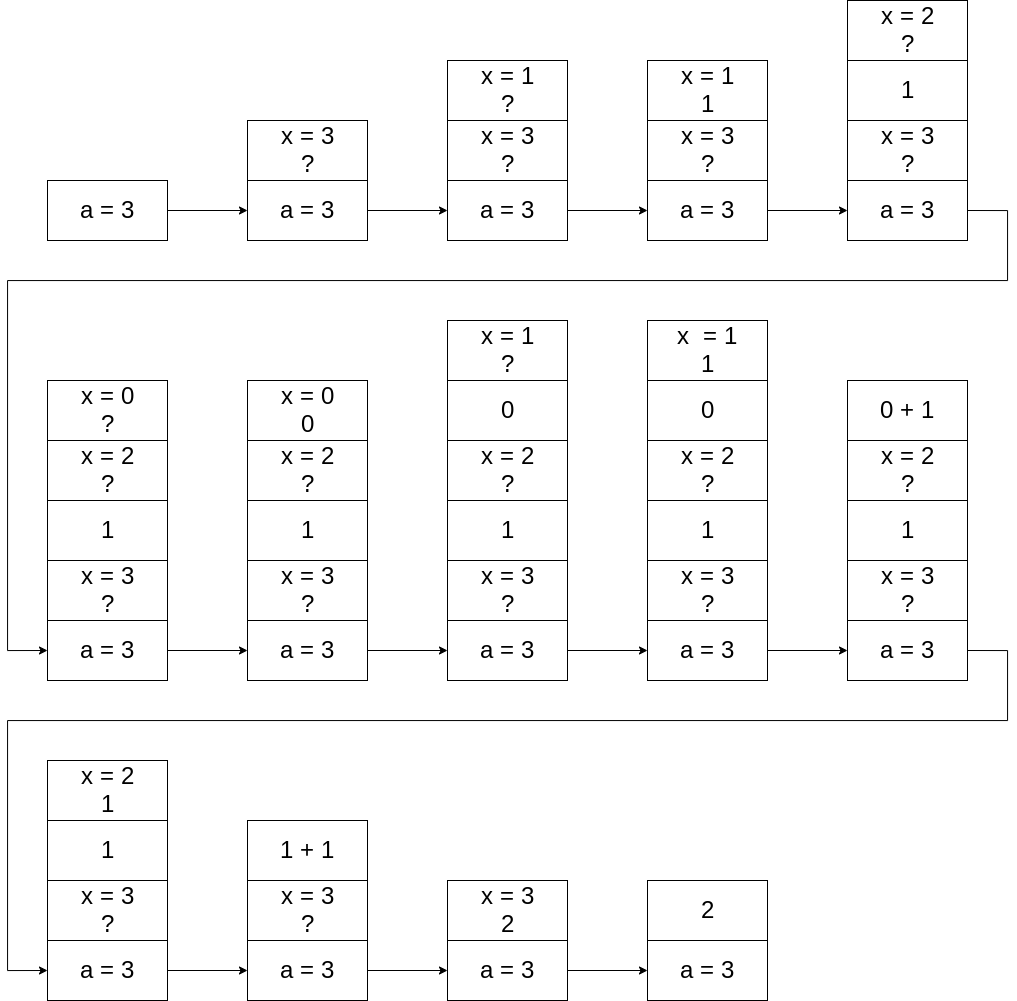
\includegraphics[width=\linewidth]{01.png}
\end{figure}


\end{document}
